\documentclass{article}

% set font encoding for PDFLaTeX or XeLaTeX
\usepackage{ifxetex}
\ifxetex
  \usepackage{fontspec}
\else
  \usepackage[T1]{fontenc}
  \usepackage[utf8]{inputenc}
  \usepackage{lmodern}
\fi
\usepackage{graphicx}
\usepackage{float}

% used in maketitle
\title{Reporte de Actividad 3}
\author{Rolando A. Fimbres G.}
\date{13 de Febrero de 2018}

% Enable SageTeX to run SageMath code right inside this LaTeX file.
% documentation: http://mirrors.ctan.org/macros/latex/contrib/sagetex/sagetexpackage.pdf
% \usepackage{sagetex}

\begin{document}
\maketitle
\section{Introducción}
La actividad de ésta sesión se trató acerca del manejo de datos. Con los conocimientos de la actividad anterior nos fue posible escribir el código adecuado en python, para poder interpretar, por medio de gráficas archivos de texto. Los archivos de texto analizado fueron de datos de sondeo atmosférico de la Universidad de Wyoming.
\section{Fundamentos}
En ésta ocasión se creó una nueva carpeta para la actividad desde la terminal. Ahí mismo abrimos un jupyter notebook, donde efectuamos el análisis. Después procedemos a habilitar algunos de los paquetes que ofrece python. Uno de ellos \textit{pandas} que son herramientas para el análisis de datos para lenguaje python. Otro es \textit{numpy} que consiste en una biblioteca de funciones matemáticas de alto nivel, así como soporte para vectores y matrices. Finalmente \textit{mathplotlib} una biblioteca para crear gráficas en 2D de buena calidad.
\section{Análisis de Datos}
En mi caso tomé los archivos de texto de una estación localizada en Tabuk, Arabia Saudita; los datos de junio y diciembre fueron tomados tanto como de 00Z como 12ZZ. Comencé leyendo cada archivo como csv siendo limitado segun sus filas. Después tomé un rapido vistazo con la función \textit{head()}. Después se crearon dos gráficas de presión contra altura. Más adelante graficas de temperatura y temperatura del rocío contra el tiempo. Después de rapidez de los vientos. Finalizando con gráficas de humedad relativa en función de la altura.
\section{Resultados}

    \begin{figure}[H]
        \centering
        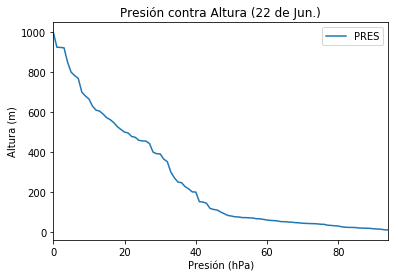
\includegraphics[width=\linewidth]{paj.png}
    \end{figure}
    \begin{figure}[H]
        \centering
        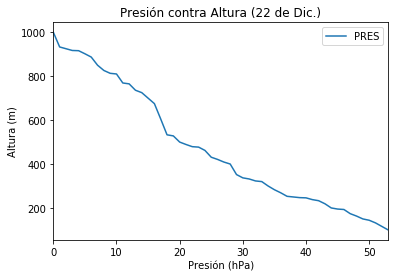
\includegraphics[width=\linewidth]{pad.png}
    \end{figure}
    \begin{figure}[H]
        \centering
        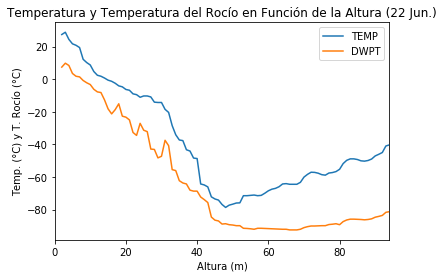
\includegraphics[width=\linewidth]{ttrj.png}
    \end{figure}
    \begin{figure}[H]
        \centering
        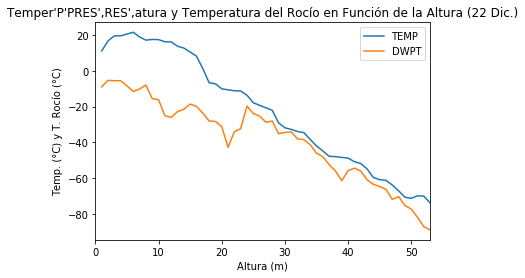
\includegraphics[width=\linewidth]{ttrd.png}
    \end{figure}
    \begin{figure}[H]
        \centering
        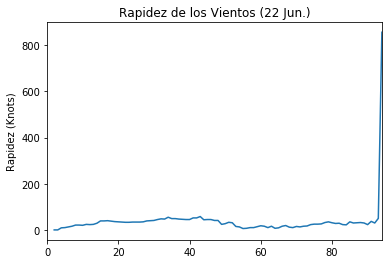
\includegraphics[width=\linewidth]{vj.png}
    \end{figure}
     \begin{figure}[H]
        \centering
        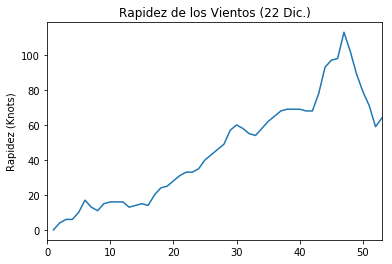
\includegraphics[width=\linewidth]{vd.png}
    \end{figure}
     \begin{figure}[H]
        \centering
        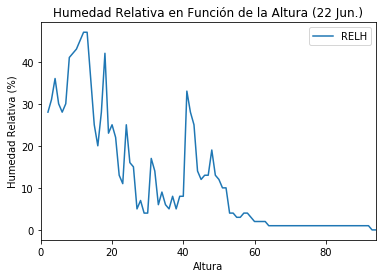
\includegraphics[width=\linewidth]{hj.png}
    \end{figure}
     \begin{figure}[H]
        \centering
        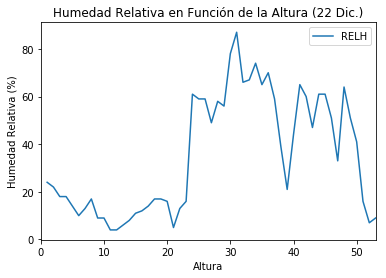
\includegraphics[width=\linewidth]{hd.png}
    \end{figure}
    
\section{Conclusión}
La realización de ésta práctica me ayudó para comprender más el lenguaje python y la utilización de los paquetes adecuados dependiendo de los datos a tratar. El conocer el uso de paquetes como mathplotlib y pandas permite el estudio de datos; lo cual es muy importante pues su análisis constituye una base importante en la labor científica. 
\section{Bibliografía}

\section{Apéndice}
1.-¿Cuál es tu opinión general de ésta actividad?\\
\\
La actividad me gustó porque pude hacer más uso de los paquetes para análisis de datos de python.\\
\\
2.-¿Qué fue lo que más te agradó? ¿Lo que menos te agradó?\\
\\
Lo que más me agrado fue ver que se graficaba correctamente lo que escribía. Lo que menos me agradó fué que tuve que restringir algunos de los renglones de la base de datos para leerlos correctamente. Me tomó más tiempo de lo que hubiera querido encontrar la función para hacerlo.\\
\\
3.-¿Qué consideras que aprendiste en ésta actividad?\\
\\
Considero que aprendí a hacer mejor uso de los paquetes y bibliotecas de python vistos en la actividad.\\
\\
4.-¿Qué le faltó? ¿Qué le sobró?\\
\\
A mi parecer no le faltó ni sobró nada.\\
\\
5.-¿Qué mejoras sugieres a la actividad?\\
\\
Añadiría sugerencias acerca de cómo abordar algunos puntos, así como ejemplos.\\
\\
\end{document}
